
\documentclass[11pt]{article}

\usepackage{UF_FRED_paper_style}

\usepackage{apacite}
\usepackage{txfonts}
\usepackage{tikz}
\usepackage{amsthm}
\usepackage[capposition=top]{floatrow}
\usepackage[format=plain,
            labelfont={it}, singlelinecheck=false,
            justification = raggedright,
            labelsep = period,
            figureposition=top]{caption}
\usepackage{algorithm}
\usepackage{algpseudocode}
\usepackage{amssymb}
\usepackage{amsmath}
%\usepackage{MnSymbol}


\makeatletter
\newcommand\multiline[1]{\parbox[t]{\dimexpr\linewidth-\ALG@thistlm}{#1}}
\makeatother

% (in)dependence symbol
\usepackage{unicode-math}

\makeatletter
\newcommand*{\indep}{%
  \mathbin{%
    \mathpalette{\@indep}{}%
  }%
}
\newcommand*{\nindep}{%
  \mathbin{%                   % The final symbol is a binary math operator
    %\mathpalette{\@indep}{\not}% \mathpalette helps for the adaptation
    \mathpalette{\@indep}{/}%
                               % of the symbol to the different math styles.
  }%
}
\newcommand*{\@indep}[2]{%
  % #1: math style
  % #2: empty or \not
  \sbox0{$#1\perp\m@th$}%        box 0 contains \perp symbol
  \sbox2{$#1=$}%                 box 2 for the height of =
  \sbox4{$#1\vcenter{}$}%        box 4 for the height of the math axis
  \rlap{\copy0}%                 first \perp
  \dimen@=\dimexpr\ht2-\ht4-.2pt\relax
      % The equals symbol is centered around the math axis.
      % The following equations are used to calculate the
      % right shift of the second \perp:
      % [1] ht(equals) - ht(math_axis) = line_width + 0.5 gap
      % [2] right_shift(second_perp) = line_width + gap
      % The line width is approximated by the default line width of 0.4pt
  \kern\dimen@
  \ifx\\#2\\%
  \else
    \hbox to \wd2{\hss$#1#2\m@th$\hss}%
    \kern-\wd2 %
  \fi
  \kern\dimen@
  \copy0 %                       second \perp
}
\makeatother
%%%%%%%%%%%%%
% dotted underline
\newcommand{\udensdot}[1]{%
    \tikz[baseline=(todotted.base)]{
        \node[inner sep=1pt,outer sep=0pt] (todotted) {#1};
        \draw[densely dotted, thick] (todotted.south west) -- (todotted.south east);
    }%
}%



\theoremstyle{definition}
\newtheorem{definition}{Definition}
%use next two lines instead for non-italic alternative
%\newtheorem{preremark}{Definition}
%\newenvironment{mydef}{\begin{preremark}\upshape}{\end{preremark}}

%% ===============================================
%% Setting the line spacing (3 options: only pick one)
% \doublespacing
% \singlespacing
\onehalfspacing
%% ===============================================

\setlength{\droptitle}{-5em} %% Don't touch

% %%%%%%%%%%%%%%%%%%%%%%%%%%%%%%%%%%%%%%%%%%%%%%%%%%%%%%%%%%
% SET THE TITLE
% %%%%%%%%%%%%%%%%%%%%%%%%%%%%%%%%%%%%%%%%%%%%%%%%%%%%%%%%%%

% TITLE:
\title{Research Report}

% AUTHOR:
\author{Kyuri Park\\% Name author
    \href{mailto:k.park@uu.nl}{\texttt{k.park@uu.nl}}} %% Email
    
% DATE:
\date{\today}

% %%%%%%%%%%%%%%%%%%%%%%%%%%%%%%%%%%%%%%%%%%%%%%%%%%%%%%%%%%
% %%%%%%%%%%%%%%%%%%%%%%%%%%%%%%%%%%%%%%%%%%%%%%%%%%%%%%%%%%
\begin{document}

{\setstretch{.8}
\maketitle

\noindent
\textit{\textbf{Keywords: }%
Cyclic causal discovery (CCD); Cyclic causal inference (CCI); Maximal ancestral graph (MAG); Partial ancestral graph (PAG)} \\ %% <-- Keywords HERE!
\noindent
}

% %%%%%%%%%%%%%%%%%%%%%%%%%%%%%%%%%%%%%%%%%%%%%%%%%%%%%%%%%%
% %%%%%%%%%%%%%%%%%%%%%%%%%%%%%%%%%%%%%%%%%%%%%%%%%%%%%%%%%%
% BODY OF THE DOCUMENT
% %%%%%%%%%%%%%%%%%%%%%%%%%%%%%%%%%%%%%%%%%%%%%%%%%%%%%%%%%%
% %%%%%%%%%%%%%%%%%%%%%%%%%%%%%%%%%%%%%%%%%%%%%%%%%%%%%%%%%%

% --------------------
\section{Introduction}
% --------------------

\subsection{Background}

A fundamental task in various disciplines of science is to find underlying mechanisms, so-called causal relations, in the phenomena of interest. In psychology, for example, one of the core questions is how the psychopathology comes about and network theory of psychopathology posits that mental disorder is produced by a system of direct and mutual causal interactions between symptoms \citep{BorsboomCramer2013}. In practice, empirical researchers aim to gain insight into these causal relations by fitting statistical network models to observational data \citep{robinaugh2020}. However, it has been shown that statistical network models are likely to perform poorly for discovering causal relationships, since relations in the network can be produced by unwittingly conditioning on common effects between other variables or induced by unobserved confounding variables. \citep{Ryan2022}.

\cite{Ryan2022} suggest that network models could in principle be replaced by using purpose-built causal discovery (CD) algorithms developed in the field of graphical causal modeling \citep{spirtes_algorithm_1991}. However, the most popular and well-studied CD algorithms assume that causal relationships are acyclic \citep{Glymour2019}; if X causes Y then Y does not cause X. This is counter to our expectations in psychological settings, necessitating the use of cyclic causal discovery (CCD) algorithms \citep{richardson1996}. Cyclic causal discovery algorithms are, however, more difficult to apply and interpret \citep{Bongers2021}, and little research has been done on their performance in settings we would expect to encounter in psychological research.

\subsection{Current Project}
We choose four algorithms for this study that can handle cyclic structure and/or latent variable as well as selection bias: cyclic causal discovery (CCD), cyclic causal inference (CCI), fast causal inference (FCI), greedy fast causal inference (GFCI). The first three algorithms are constraint-based methods, while GFCI is a hybrid algorithm as it uses both constraint-based and score-based methods. A constraint-based method utilizes conditional independence tests trying to eliminate edges that are inconsistent with the observed constraints starting from a fully-connected graph. A score-based method on the other hand searches over the space of possible graphs and add/remove edges trying to maximize a score that reflects how well the graph fits the data, starting from an empty graph. 
% explain constrain, score-based.

% To reflect the study designs that are often encountered in psychological network research, we employ simulations where we vary sample sizes, density (i.e., number of causal relationships), and presence of unobserved confounders. We expect most algorithms would perform well in situations where the sample size is sufficiently large, density is low, and unobserved confounders are absent. Such situations are rare in psychological research, which brings the challenge and hence it is of interest to investigate the performance of algorithms under the typical psychological settings (i.e., low sample size, high density, presence of confounders). Thus, the research question this project addresses is: \textit{how well do cyclic causal discovery algorithms perform in typical psychological research contexts?}\\

The goal of this study is threefold: (a) we want to provide an overview of a set of causal discovery algorithms that are potentially suitable for typical observational psychological data; (b) we want to investigate how well each of these algorithms can estimate causal relations by means of a simulation study; (c) we want to test these algorithms by applying them to empirical data.

\subsection{Graphical Models}
A graphical model is a set of multivariate joint distributions that show certain conditional (in)dependencies among random variables. Each model is associated with a graph $G = (V, E)$, where $V$ represents a set of vertices (variables) and $E$ represents a set of edges between each pair of vertices. Graphical models can capture the probabilistic and causal properties of multivariate distributions, hence called causal models, under two assumptions: \textit{causal Markov assumption} stating that any changes in causal structure from the graph imply corresponding changes in the probability distribution and \textit{faithfulness assumption}, which states the reverse such that any changes in conditional independencies imply changes in the associated graph structure.

The simplest and most well-known case of a causal graph is \textit{directed acyclic graph} (DAG), which consists of directed edges with a straightforward interpretation (e.g., $X\rightarrow Y$ denotes a direct causal relationship such that X causes Y). DAGs, however, have limitations on representing causal structure with either latent variables (i.e., they assume causal sufficiency, an assumption that there exists no unobserved latent variables) or cycles (i.e., they assume there exists no feedback loops). In this study, we mainly deal with maximal ancestral graph (MAG), maximal almost ancestral graph (MAAG), and partial ancestral graph (PAG), which are the output of the considered algorithms. 

Ancestral graphs are an extension of DAGs that can represent causal structures when the underlying data generating mechanism involves unobserved latent confounders and selection variables (Spirtes \& Richardson, 2002). Correspondingly, ancestral graphs can have following edge types besides the directed edges ($\rightarrow$): bidirected edges ($\leftrightarrow$) to represent the presence of latent variables and undirected edges ($\textendash$) to represent the presence of selection variables. The orientation of edges in ancestral graph represents causal ancestry. For example, a directed edge $X \rightarrow Y$ denotes that $X$ is an ancestor of $Y$, but the relation is not necessarily direct, and vice versa in case of $X \leftarrow Y$. 

A \textit{maximal ancestral graph} (MAG) is an ancestral graph that satisfies pairwise Markov property, i.e., every missing edge corresponds to a conditional independence relation. In other words, if two vertices are not adjacent in a MAG, then there is a set of some other vertices that \textit{m-separates} the two (see Definition~\ref{def: def2} and \ref{def: def3}). 

Different MAGs representing the same set of \textit{m-separation}, are summarized within a Markov equivalence class, which is represented by \textit{partially ancestral graph} (PAG). A PAG for graph $G$ contains partial information regarding ancestral relations in $G$, namely only those ancestor relations common to all members of equivalence set of $G$, $Equiv(G)$. In PAGs, edges can end with a circle ($\circ$), which represents both possibilities of an arrow's head and tail. Thus, the possible types of edges in PAGs are as follows: $\rightarrow, \leftrightarrow, \textendash, \multimapinv>, \multimapinv, \multimapboth$. %find the latex arrow with circle end. 

An \textit{almost ancestral} graph is the graph that satisfies only the first two conditions of ancestral graph (see Definition~\ref{def: def1}). A \textit{maximal almost ancestral graph} (MAAG) is hence an almost ancestral graph in which pairwise Markov property holds. Note that MAAG does not necessarily preserve the \textit{m-separation} relations between observed variables given selection variables in a graph $G$, meaning that MAAG itself may not have a global Markov property?..... As in PAGs, MAAGs can have 6 different edge types ($\rightarrow, \leftrightarrow, \textendash, \multimapinv>, \multimapinv, \multimapboth$), where $\circ$ again implies that the endpoint cannot be determined.


\begin{definition} [Ancestral graph] \label{def: def1}
A graph model is \textbf{ancestral} if the following three condtions hold:
1. There is no directed cycle. (A directed cycle occurs when $B \rightarrow A$ and $A \in Ancestor(B)$.\\
2. There is no almost directed cycle. (An almost directed cycle occurs when $B \leftrightarrow A$ and $A \in Ancestor(B)$.\\
3. If there is an undirected edge $V_1 - V_2$, then $V_1$ and $V_2$ have no incoming arrowheads.
\end{definition}

\begin{definition} [m-separation] \label{def: def2}
In an ancestral graph, $V_1$ and $V_2$ is \textbf{m-separated} given a set of vertices $Z\ (V_1, V_2 \notin Z)$ if there is no active path between $V_1$ and $V_2$ relative to $Z$. 
\end{definition}

\begin{definition} [maximality] \label{def: def3}
An ancestral graph is said to be \textbf{maximal} if for any two non-adjacent vertices, there is a set of vertices that \textit{m-separates} them.
\end{definition}

\begin{definition} [Markov property] \label{def: def4}


\end{definition}


\begin{figure}[H]
    \centering
        \caption{Overview of causal graphical models.}
        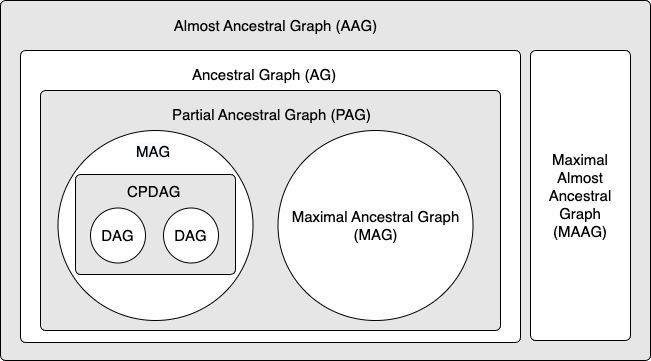
\includegraphics[scale=.6]{figures/diagram.png}
        \vspace{3mm}
        \caption*{\textit{Note.} DAG = Directed acyclic Ggraph, CPDAG = Completed partially directed acyclic Graph}
    \label{fig:1}
\end{figure}

\begin{figure}[H]
    \centering
        \caption{Example graphical models.}
        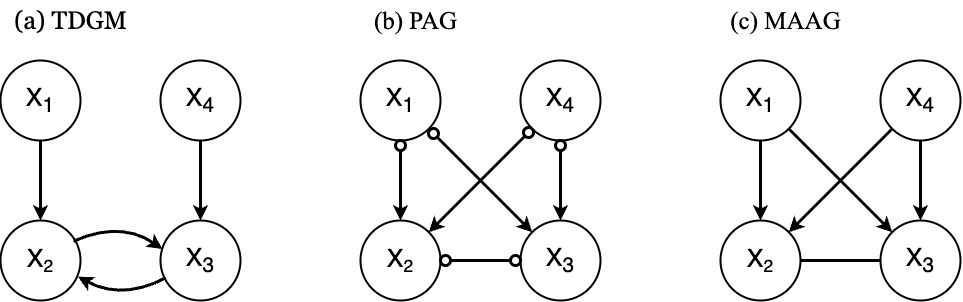
\includegraphics[scale=.4]{figures/graphs.png}
        \vspace{3mm}
        \caption*{\textit{Note.}(a) is the example true data generating model, $G$. (b) is partial ancestral graph of $G$. (c) is the associated MAAG of $G$.}
    \label{fig:2}
\end{figure}



\subsection{Overview of Algorithms}
\subsubsection{Cyclic Causal Discovery (CCD)}

CCD describe (Richardson 2013 paper)
(Algorithm logics) + output interpretation
Richardson keeps saying d-separtion..instead of m-separtion.. confusing?!

% CCD algorithm
\begin{algorithm}
\caption{Cyclic Causal Discovery (CCD)}
 \hspace*{\algorithmicindent} \textbf{Input:} A conditional independent oracle\footnote{explain orcale} for a distribution $\mathcal{P}$, satisfying global directed Markov property and faithfulness conditions with respect to a directed graph $\mathcal{G}$ with vertex set $\mathcal{V}$. \\
 \hspace*{\algorithmicindent} \textbf{Output:} A PAG $\Psi$ for the Markov equivalence class $\text{Equiv}(\mathcal{G})$.
\begin{algorithmic}[1]
\State \textit{\textbf{Step 1.}} Form a complete graph ($\Psi$) with the edge $\multimapboth$ between every pair of vertices in $\mathcal{V}$.
    \State $n = 0$
    \Repeat
        \Repeat
            \State \multiline{Select an ordered pair of variables $X$ and $Y$ that are adjacent in $\Psi$ such that the number of vertices in $\mathbf{Adjacent}(\Psi ,X)\footnote{explain Adjacency}\backslash\{Y\} \ge n$, and select a subset $\mathcal{S}$ of $\mathbf{Adjacent}(\Psi ,X) \backslash \{Y\}$ with $n$ vertices. \\
            If $X \indep Y \mid \mathcal{S}$, then delete the edge $X \multimapboth Y$ and record $\mathcal{S}$ in $\mathbf{Sepset} \langle X,Y \rangle$\footnote{explain Sepset} and $\mathbf{Sepset}\langle X,Y \rangle$.}
            \vspace{.1mm}
        \Until{ \multiline{all pairs of adjacent variables $X$ and $Y$ such that  the number of vertices in $\mathbf{Adjacent}(\Psi ,X)\backslash\{Y\} \ge n$ and all sets $\mathcal{S}$ such that the number of vertices in $\mathcal{S} = n$ have been tested.\\
        $n = n + 1;$}}
        \vspace{.1mm}
    \Until{ for all ordered pairs of adjacent vertices $X$ and $Y$, $\mathbf{Adjacent}(\Psi ,X)\backslash\{Y\} < n$}.
\State \textit{\textbf{Step 2.}} For each triple of vertices $A, B, C$ such that each of the pair of $A, B$ and the pair $B, C$ are adjacent in $\Psi$ but the pair $A, C$ are not adjacent in $\Psi$, then:
    \State (i) orient $A *-*B*-*C$ as $A \rightarrow B \leftarrow C$ \textit{iff} $B \notin \mathbf{Sepset}\langle A, B \rangle$.
    \State (ii) orient $A *-*B*-*C$ as $A *-* \underline{B}*-*C$ \textit{iff} $B \in \mathbf{Sepset}\langle A, B \rangle$.

\State \textit{\textbf{Step 3.}} For each triple of vertices $A, X, Y$ in $\Psi$ such that (a) $A$ is not adjacent to $X$ or $Y$, (b) $X$ and $Y$ are adjacent, (c) $X \notin \mathbf{Sepset}\langle A, Y \rangle$ , then orient $X *-* Y$ as $X \leftarrow Y$ if $A \nindep X \mid \mathbf{Sepset}\langle A, Y \rangle$.

\State \textit{\textbf{Step 4.}} For each vertex $V$ in $\Psi$ form the following set: $X \in \mathbf{Local}(\Psi, V)\footnote{explain Local}$ or there is a vertex $Y$ such that $X \rightarrow Y \leftarrow V$ in $\Psi$\footnote{$\mathbf{Local}(\Psi, V)$ is not recalculated as the algorithm progresses.}.
\State $m = 0$
    \Repeat
        \Repeat 
            \State \multiline{Select an ordered triple \<$A$, $B$, $C$\> such that $A \rightarrow B \leftarrow C$, $A$ and $C$ are not adjacent, and $\mathbf{Local}(\Psi, A) \backslash \{B, C\}$ has $\ge m$ vertices.\\
            Select a set $T \subseteq \mathbf{Local}(\Psi, A) \backslash \{B, C\}$ with $m$ vertices. If $A \indep C \mid T \cup \{B\}$, then orient $A \rightarrow B \leftarrow C$ as $A \rightarrow \udensdot{B} \leftarrow C$ and record $T \cup \{B\}$ in $\mathbf{Supset} \langle A, B, V \rangle$.}
            \vspace{.1mm}
        \Until \multiline{for all triples such that $A \rightarrow B \leftarrow C$ (not $A \rightarrow \udensdot{B} \leftarrow C$), $A$ and $C$ are not adjacent, $\mathbf{Local}(\Psi, A) \backslash \{B\}$ has $\ge m$ vertices, every subset $T$ with $m$ vertices has been considered.}
        \vspace{.1mm}
        \State $m = m + 1;$
    \Until \multiline{all ordered triples \<$A$, $B$, $C$\> such that $A \rightarrow B \leftarrow C$, $A$ and $C$ are not adjacent, are such that $\mathbf{Local}(\Psi, A) \backslash \{B\}$ have $< m$ vertices.}
\vspace{.1mm}
\State \textit{\textbf{Step 5.}} If there is a quadruple $A$, $B$, $C$, $D$ in $\Psi$ of distinct vertices such that:\\ 
(i) $A \rightarrow \udensdot{B} \leftarrow C$,\\
(ii) $A \rightarrow D \leftarrow C$ or $A \rightarrow \udensdot{D} \leftarrow C$,\\
(iii) $B$ and $D$ are adjacent,\\
then orient $B *-* D$ ad $B \rightarrow D$ in $\Psi$ if $D \notin \mathbf{Subset}\langle A, B, C \rangle$. Else orient $B *-* D$ as $B *- D$ in $\Psi$.

\State \textit{\textbf{Step 6.}} For each quadruple $A$, $B$, $C$, $D$ in $\Psi$ of distinct vertices such that:\\
    (i) $D$ is not adjacent to both $A$ and $C$,\\
    (ii) $A \rightarrow \udensdot{B} \leftarrow C$,\\
    if $A \nindep D \mid \mathbf{Supset} \langle A, B, C \rangle \cup \{D\}$,
    then orient $B *-* D$ as $B \rightarrow D$ in $\Psi$.
\end{algorithmic}
\end{algorithm}

\subsubsection{Cyclic Causal Inference (CCI)}


\subsection{Trace of Algorithms}
%trace CCD
\subsubsection{CCD trace}
Given a conditional independence oracle for $\mathcal{G}$ in Figure \ref{fig:2} (a), the CCD algorithm runs as follows.

\textbf{Step 1.} As $X_1 \indep X_4 \mid \emptyset$, $X_1 \multimapboth X_4$ edge is removed and record $\mathbf{Sepset} \langle A, B \rangle = \mathbf{Sepset} \langle B, A \rangle = \emptyset$.

\textbf{Step 2.} \multiline{As $X_2 \notin \mathbf{Sepset} \langle X_1, X_4 \rangle$, orient $X_1 \rightarrow X_2 \leftarrow X_4$. As $X_3 \notin \mathbf{Sepset} \langle X_1, X_4 \rangle$, orient $X_1 \rightarrow X_3 \leftarrow X_4$.}

\textbf{Step 4.} \multiline{As $X_1 \indep X_4 \mid \{X_2, X_3\}$, orient $X_1 \rightarrow \udensdot{$X_2$} \leftarrow X_4$ and $X_1 \rightarrow \udensdot{$X_3$} \leftarrow X_4$.\\
Record $\mathbf{Supset}\langle X_1 X_2 X_4 \rangle = \{X_2, X_3\}$ and $\mathbf{Supset}\langle X_1 X_3 X_4 \rangle = \{X_2, X_3\}$.}
\vspace{.1mm}

\textbf{Step 5.} \multiline{There is a quadruple such that $X_1 \rightarrow \udensdot{$X_2$} \leftarrow X_4$, $X_1 \rightarrow \udensdot{$X_3$} \leftarrow X_4$, $X_2 \multimapboth X_3$. \\
As $X_2 \in \mathbf{Supset} \langle X_1 X_3 X_4 \rangle$, orient $X_2 \multimap X_3$.\\
As $X_3 \in \mathbf{Supset} \langle X_1 X_2 X_4 \rangle$, orient $X_2  - X_3$.}
\vspace{.1mm}

Note that \textbf{step 3} and \textbf{step 4} do not perform any orientation in this case.

\begin{figure}[H]
    \centering
        \caption{Trace of CCD algorithm.}
        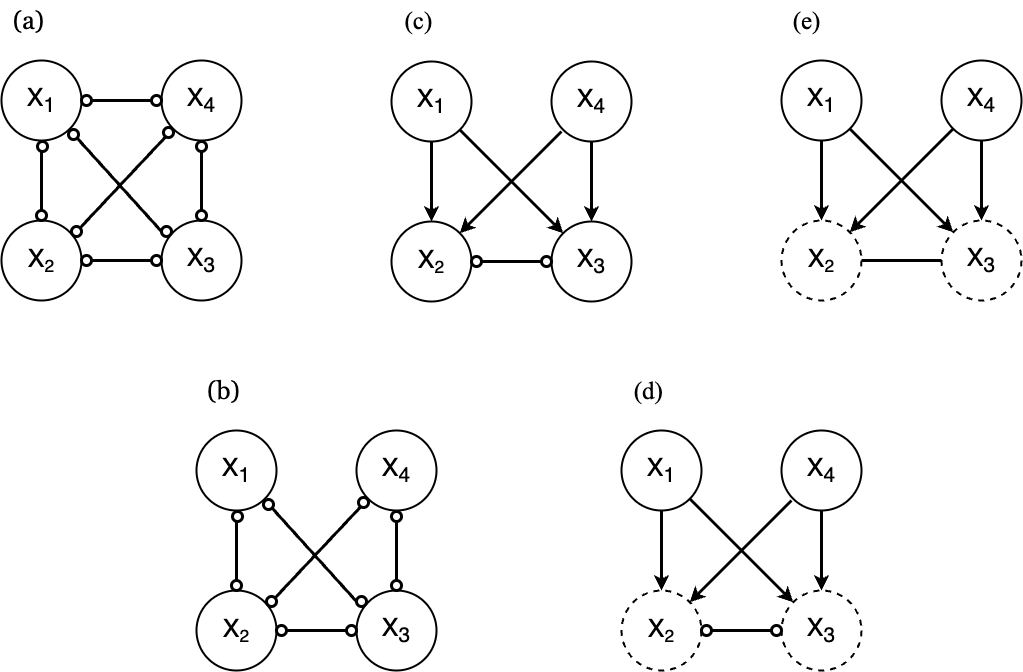
\includegraphics[scale=.3]{figures/ccdtrace.png}
    \label{fig:3}
\end{figure}

\begin{figure}[H]
    \centering
        \caption{Trace of CCI algorithm.}
        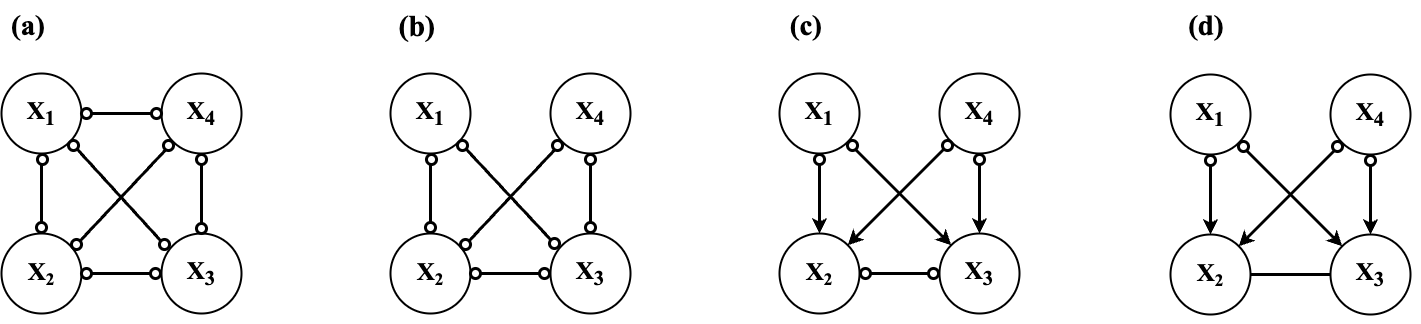
\includegraphics[scale=.3]{figures/ccitrace.png}
    \label{fig:3}
\end{figure}



\subsection{Interpretation of Outputs}

Mention PAG from CCD slightly differs from typical PAGs:
1. assume causal sufficiency: $\leftrightarrow, \circ\rightarrow$ do not occur.
2. has dottedunderline..

\begin{figure}[H]
    \centering
        \caption{The causal landscape.}
        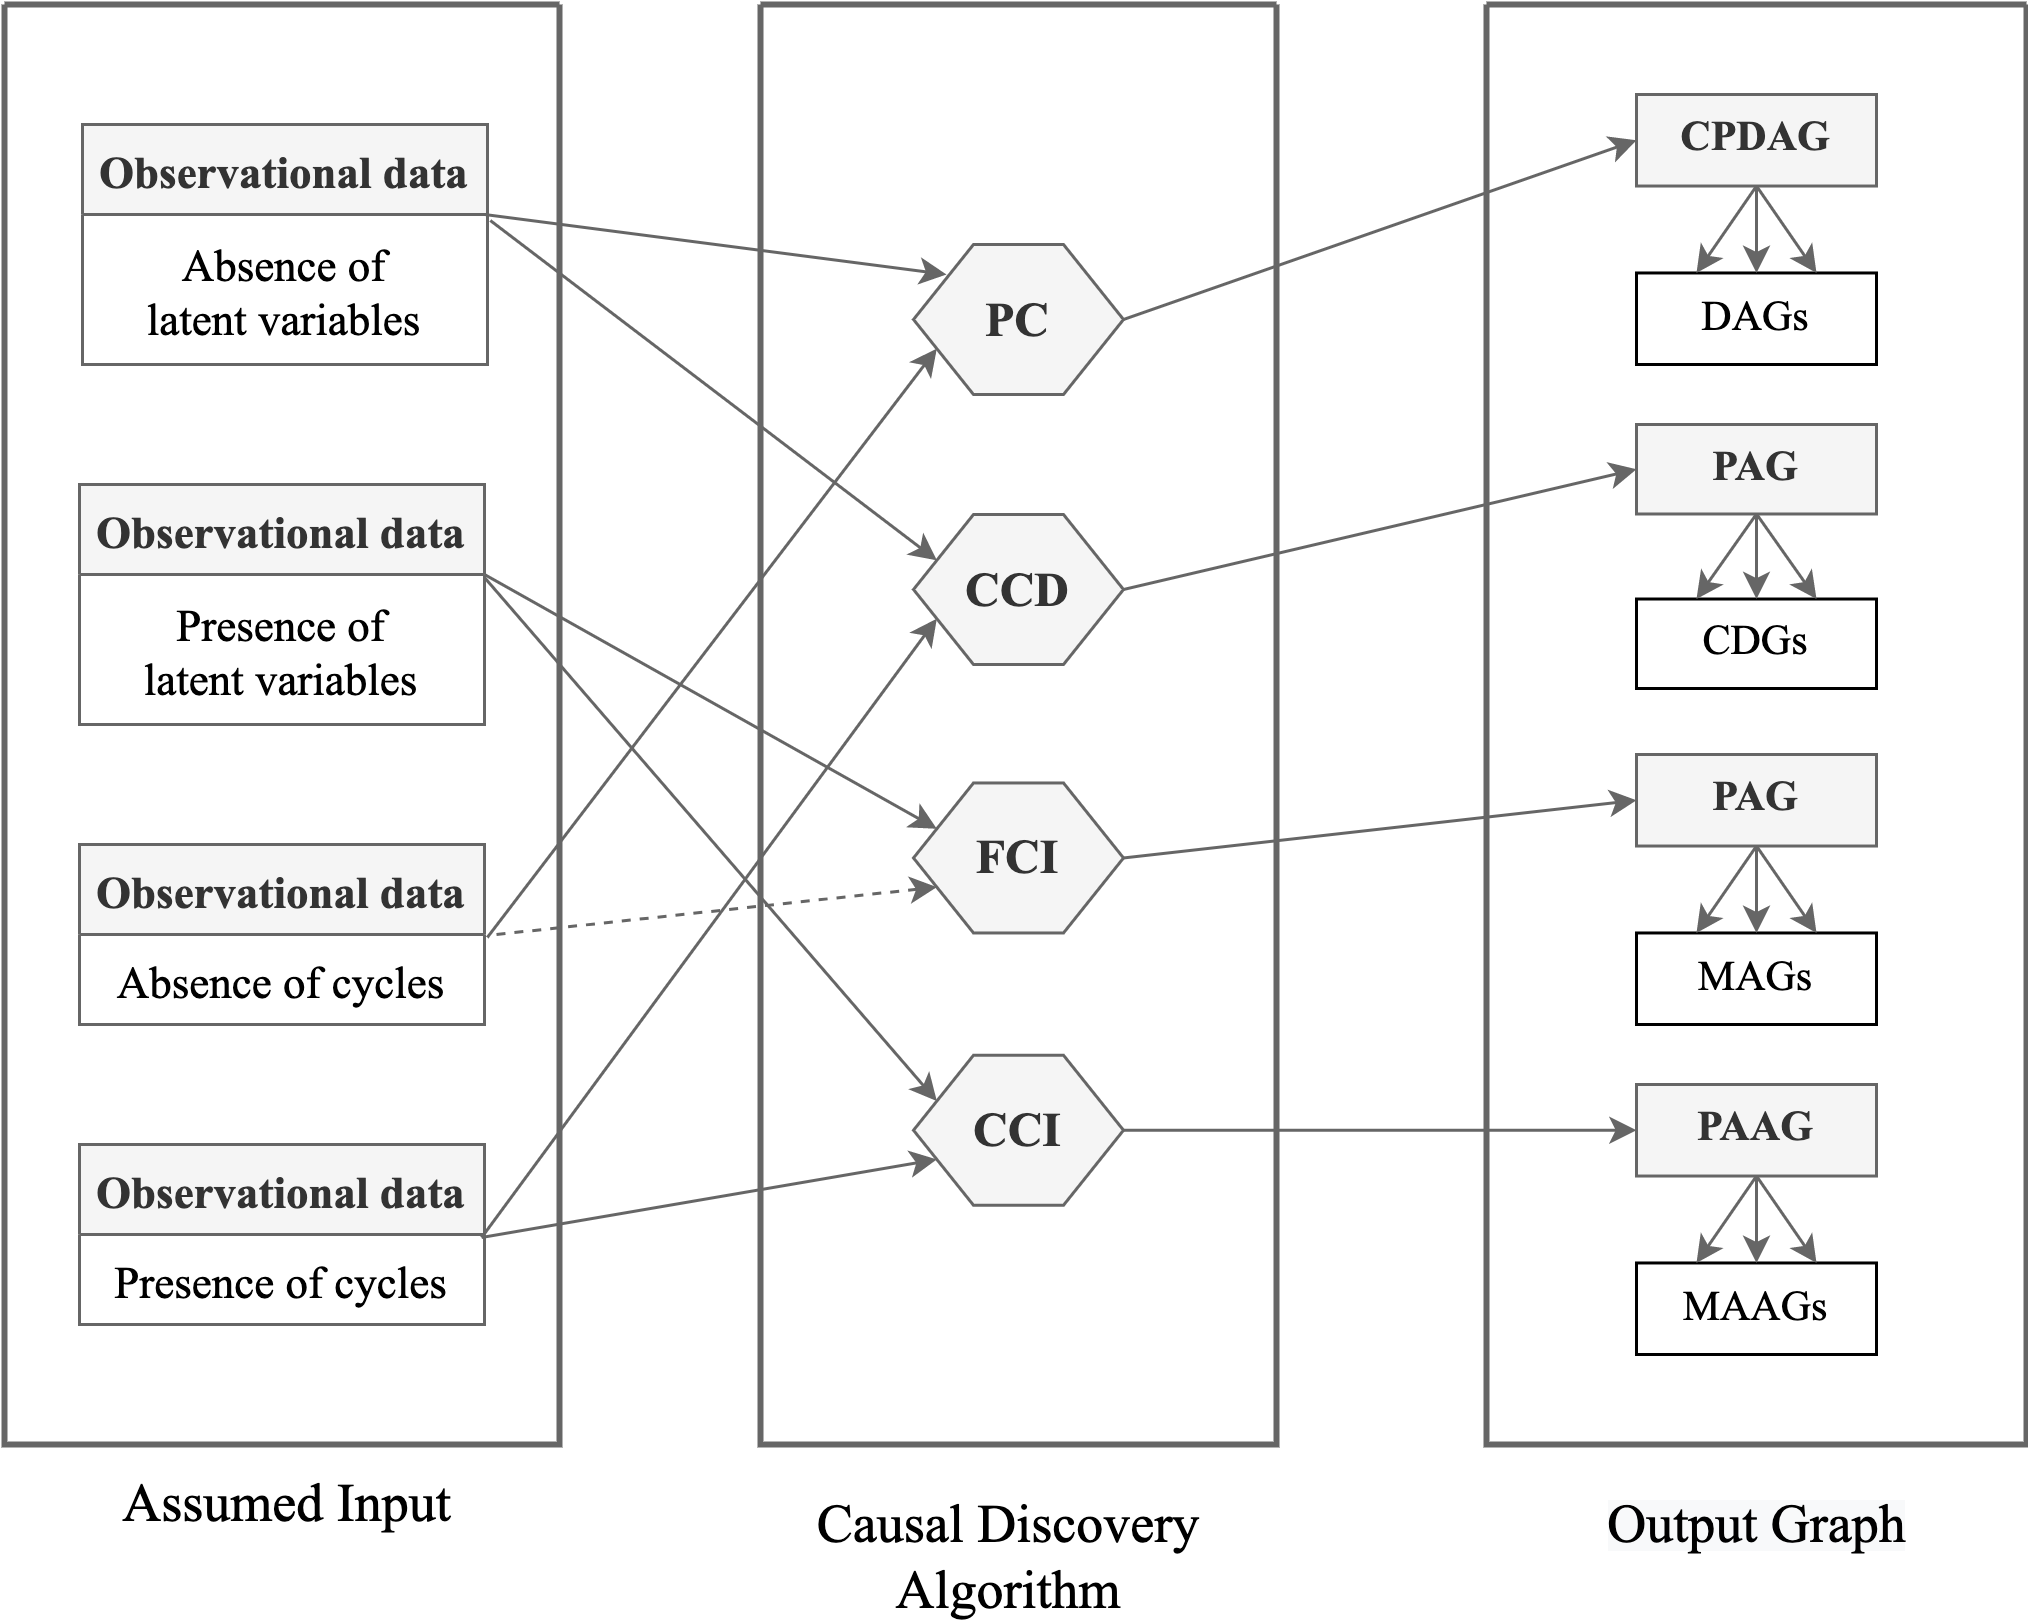
\includegraphics[scale=.6]{figures/landscape.png}
    \label{fig:4}
\end{figure}


\subsection{Graphical Models}
MAG = Mixed Ancestral Graph (Spirtes, Glymour \& Scheines, 2000)

MAG = Maximal Ancestral Graph \\
MAGs are an extension of DAGs that allow modelling of causally insufficient systems (i.e., systems with latent confounders). They are also closed under marginalization.\\
Bidirectional edges mean that there is a latent confounder; X <-> Y means neither X causes Y nor Y causes X.\\

Richardson and Spirtes (2002) introduce Maximal ancestral graphs and show that they form the smallest superclass of DAGs that is closed under marginalization. These are mixed graph and contained directed and bidirected edges. MAGs come with a slightly different separation criterion: \textit{m-separation}. For each DAG with hidden variables, there is a unique MAG over the observed variables that represents the same set of conditional independencies (by m-separation). This mapping is not one-to-one. Each MAG can be constructed by infinitely many different DAGs (containing an arbitrary number of hidden variables). Different MAGs representing the same m-separation, are summarized within a Markov equivalence class; this equivalence class is represented by a partially ancestral graph (PAG). In PAGS, edges can end with a circle, which represents both possibilities of an arrow's head and tail.

PAG = Partial Ancetral Graph represents the Markov equivalnce class of all the statistically equivalent MAGs by using a special notation ("o") for edge endpoints that cannot be determined. 


Richardson (1996, 1996b) introduces Partial Ancestral Graph (PAG), which represents features common to Markov equivlance classes of directed graph models (DGs) and the O-Markov equivalence class of DAGs.  

% --------------------
\section{Methodology}
% --------------------

% --------------------
\section{Results}
% --------------------


% --------------------
\section{Discussion and Conclusions}
% --------------------


% %%%%%%%%%%%%%%%%%%%%%%%%%%%%%%%%%%%%%%%%%%%%%%%%%%%%%%%%%%
% %%%%%%%%%%%%%%%%%%%%%%%%%%%%%%%%%%%%%%%%%%%%%%%%%%%%%%%%%%
% REFERENCES SECTION
% %%%%%%%%%%%%%%%%%%%%%%%%%%%%%%%%%%%%%%%%%%%%%%%%%%%%%%%%%%
% %%%%%%%%%%%%%%%%%%%%%%%%%%%%%%%%%%%%%%%%%%%%%%%%%%%%%%%%%%
\medskip

\bibliography{references.bib} 

\end{document}